%
%
%
%
\section{Unsteady Turbomachinery Flows}
\headb{Introduction}{Unsteady turbomachinery flows}
\label{unsteady_flow_intro.sec}
%
 Turbomachinery stages are designed to produce work on the fluid flow
 which passes through them. This is true for both turbine rotor blades,
 where the air flow decreases its total enthalpy in order to allow the
 blade rotation; and for compressor rotor blades, where the fluid receives
 energy from the rotation of the blade, thus increasing its total enthalpy.
 For a flow with negligible body forces, the first low of thermodynamics
 can be written as

%
\beq
  \frac{D H}{D t} = \frac{1}{\rho}\fpdt{p}
  \label{first_law.eq}
\eeq
%
 where $H$ is the total enthalpy, $p$ the pressure and $\rho$ the density
 of the fluid with $\frac{D}{D t}$ indicating the convective (or total)
 derivative.
 Equation (\ref{first_law.eq}) shows that, in order to produce work, i.e.
 changing the total enthalpy of the fluid, the fluid flow within
 turbomachinery blade rows must be unsteady. This is consistent with the
 fact that, in the case of a turbine rotor blade, where the total enthalpy
 decreases, a stationary observer would see, at a fixed viewpoint, a decreasing
 pressure with time ($\fpdt{p} < 0$) since first the pressure and then
 the suction side of the passage will go past the observer's point of view.
 This relative blade row motion is essential for turbomachines
 to produce work.

 On the other hand, the relative motion causes complicated
 unsteady interactions between adjacent blade rows which can persist
 through several stages and can cause severe vibration problems.
 The wake shed by the downstream blade is unsteady for the upstream one;
 the potential field associated with blade lifts also causes unsteadiness
 for adjacent blade rows.
 Other factors, such as aerodynamic mistuning, i.e. stator throat width
 variations due to assembly tolerances, temperature distortions, due to
 blocked burners, may also become significant in causing unsteady excitation
 forces with low-order harmonics, the so-called low engine order excitation
 (LEO).
 Blade vibration is another source of unsteadiness
 and the overall picture is further complicated because of other inherently
 unsteady phenomena such as vortex shedding, surge, stall and rotating stall,
 though some are associated with part-speed only.

 Such unsteady phenomena play a crucial role in the aeroelastic and
 aeroacoustic behaviour of the blades and they are increasingly becoming
 limiting factors in the developing improved-efficiency designs,
 especially when flexible, slender and unshrouded blades are used.
 From an industrial prospective, it is clear that there is a pressing
 need for formulating validated predictive
 models to reduce the design cycle and, consequently, cost.

 This thesis will address such a problem and focus on the numerical
 simulation of unsteady turbomachinery flows for forced response
 predictions.
%
%
%
%
\subsection{Forced response}
%
 When the rotating blades pass through flow defects created by the
 upstream and downstream blade rows, the ensuing large unsteady
 aerodynamic forces can cause excessive vibration levels, hence the term
 forced response. One of the first design steps, for minimizing the response
 levels, is the Campbell diagram of Fig. \ref{campell.fig} which
 indicates the possibility of an assembly mode being excited
 at a particular rotational speed or its multiples, the so-called
 engine order (EO) excitation.
 The Campbell diagram is a plot of the bladed disc mode family frequency
 against rotor speed, onto which the engine order lines are superimposed.
 Forced response occurs when a particular engine order and the assembly
 frequency lines cross, as indicated by circles in Fig. \ref{campell.fig}.
 For this reason, forced response is also called synchronous vibration as it
 occurs when two frequencies match.

 Forced response problems may be alleviated by reducing the
 aerodynamic forcing, or by controlling the resulting
 vibration\footnote{A way of achieving this is the use of under platform
 dampers}. It may be removed entirely by moving coincident frequencies
 out of the running range.
%
\begin{figure}[ht]
  \centerline{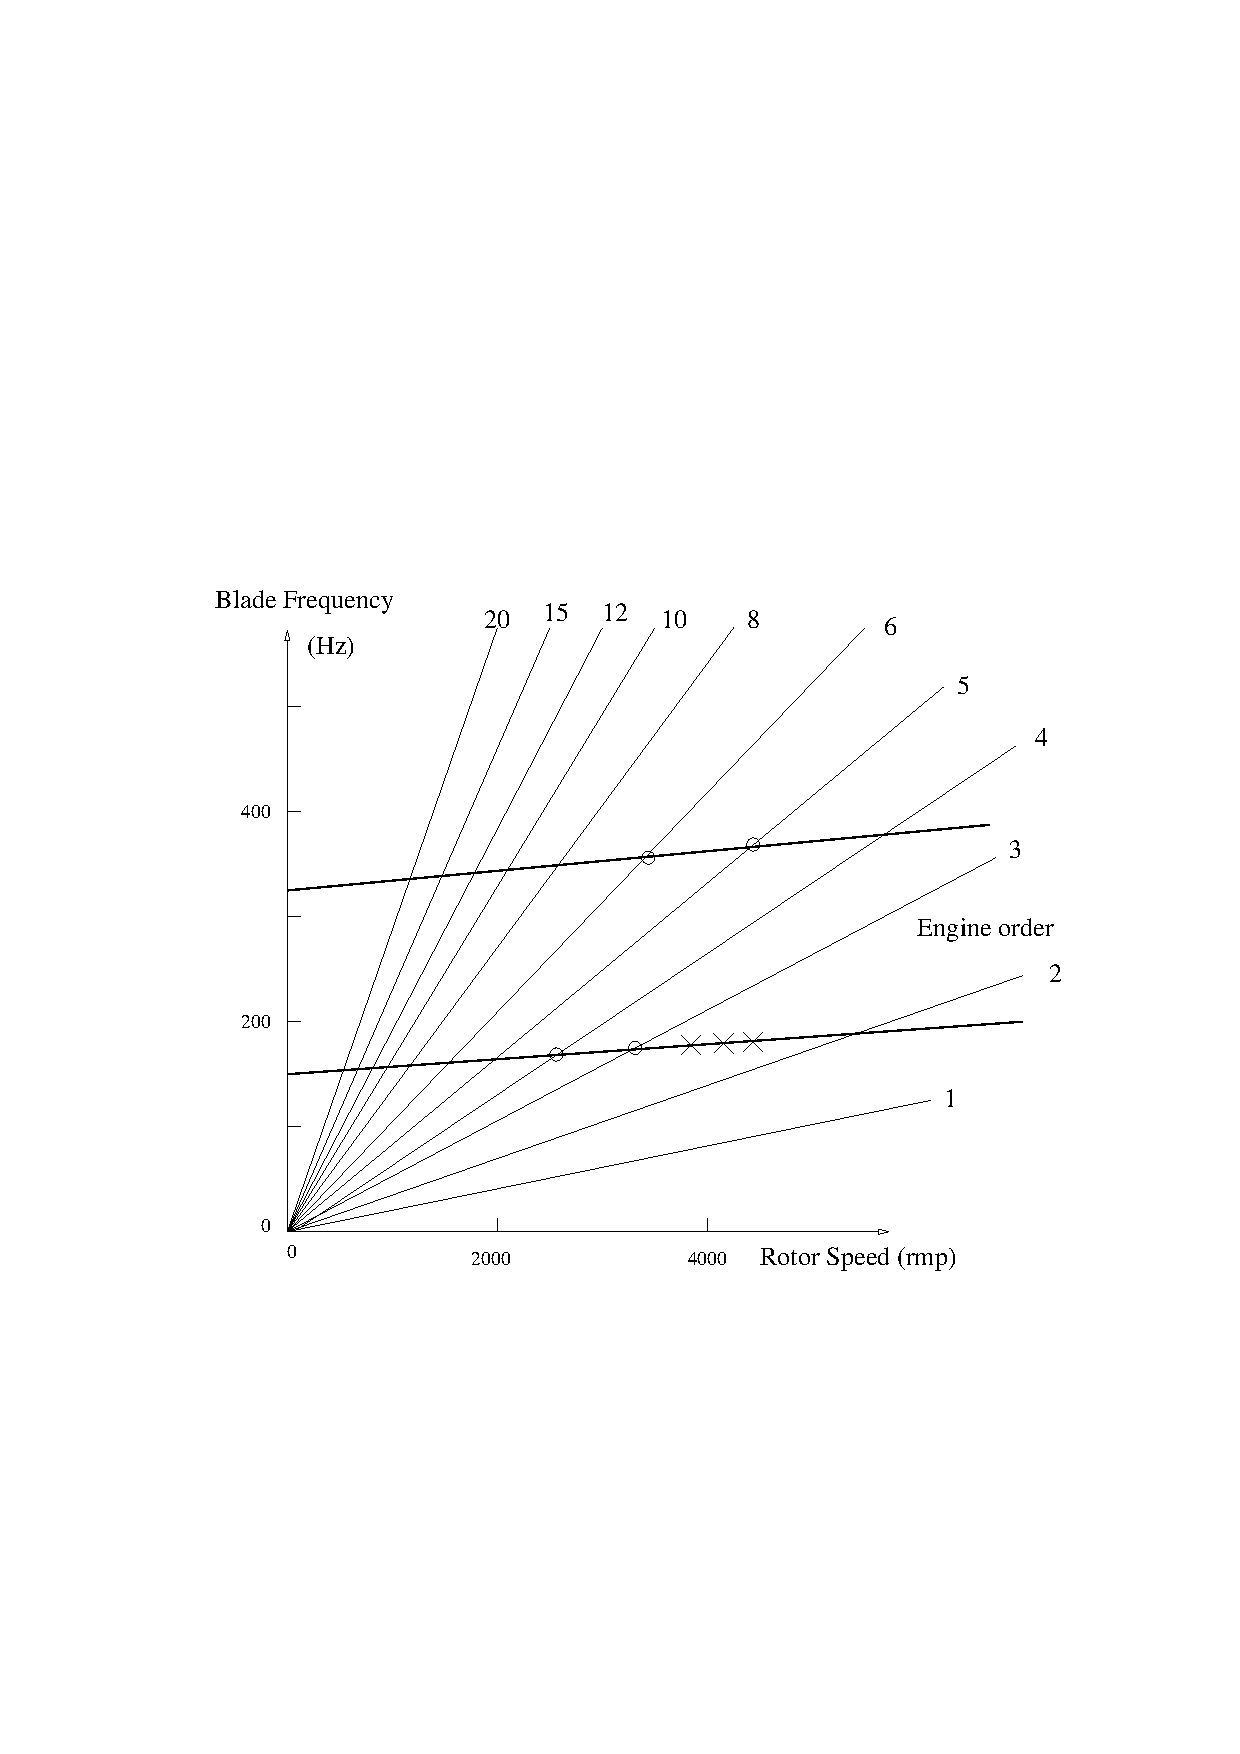
\includegraphics[width=130mm, clip=t]{CHAP_INTRO/FIGURE/campell.pdf}}
  \caption{Campbell diagram for a rotor blade (from Sisto 1987).
   x non-synchronous excitation (flutter), o forced response resonance.}
  \label{campell.fig}
\end{figure}
%
 Unfortunately, it is not usually possible to move all resonances out of the
 running range because aeroengines operate over a wide range
 of speeds and aerodynamic conditions.
 So, it is of paramount importance to be able to evaluate the unsteady
 aerodynamic loads in order to calculate the magnitude of aerodynamic
 responses for fatigue life predictions.
 This problem is usually more severe in HP turbines, where the
 blades are already under large thermal and centrifugal loading.
 Jay \& Fleeter \citeyear{Fleeter:2} give an overview of the various
 aspects of forced response investigation. An assessment of unsteady flows
 in turbines caused by the relative blade motion is given
 by Sharma et al. \citeyear{Sharma:1}.

 In aerospace engineering, it is common practice to display
 engine test results in the form of a modified Campbell diagram from
 which both flutter and forced response behaviour can be seen.
 In such cases, the out-of-plane axis represents the vibration
 amplitude and flutter is observed at nearly constant frequency,
 usually across several engine-order lines (Fig. \ref{campell.fig}).

 The main sources of unsteadiness, which can cause forced blade
 vibrations, can be due to the wake passing from upstream blade rows
 (wake-blade interaction) and the potential field of up/downstream
 blade rows.
%
\paragraph{Wake-rotor interaction.}
%
 The stator wakes, which can be
 assumed to be approximatively steady in the stator frame of
 reference, are unsteady in the rotor frame of reference since
 the rotor is moving through the wakes and, consequently, unsteady
 pressure waves are created. Although the generation of stator
 wakes is viscous phenomenon, the subsequent interaction with
 the rotor blade is primarily an inviscid process and hence can
 be modelled, as a first approximation, by the Euler equations.
 This allows two different approaches in numerical modeling.
 The first is to perform a full Navier-Stokes calculation for both the
 stator and rotor blades (Rai \citeyearNP{Rai:1,Rai:2},
 Arnone \citeyearNP{Arnone:1}. The second is to perform an unsteady
 inviscid calculation for just the rotor blade row, with the wakes
 being somehow specified as unsteady inflow boundary conditions
 (Hodson \citeyearNP{Hodson:1}, Giles \citeyearNP{Giles:2},
  Korakianitis \citeyearNP{Kora:1,Kora:2,Kora:3}).
 This latter approach is computationally much more efficient,
 but assumes that one is not concerned about the unsteady heat
 transfer and other viscous effects on the rotor blades and that the
 wake is steady in the stator frame of reference.
%
\paragraph{Potential interaction.}
%
 Such interaction cause
 unsteadiness due to the fact that the pressure in the region between
 the stator and rotor blade rows can be decomposed approximately
 into a part which is steady and uniform, a part that is
 non-uniform but steady in the rotor frame and a part that is
 non-uniform but steady in the stator frame. Therefore, as the rotor
 blades move, the stator trailing edges experience an unsteady
 pressure due to the non-uniform part that is locked to the rotors,
 and the rotor leading edges experience an unsteady pressure due to the
 non-uniform part that is locked to the stator.
 This is a purely inviscid interaction , hence the term potential interaction.
 There are again two modelling approaches:
 the first is an unsteady inviscid calculation of the stator and rotor
 blade rows (Giles \citeyearNP{Giles:3}, Suddhoo et al. \citeyearNP{Giles:11},
 Rai \citeyearNP{Rai:1,Rai:2}, Sbardella \& Peir\'{o} \citeyearNP{Luca:1}).
 The second is an unsteady inviscid calculation for just
 one of the blade rows, either the stator or the rotor, with the
 unsteady pressure being specified as boundary condition
 (Korakianitis \citeyearNP{Kora:1,Kora:2,Kora:3},
 Manwaring \& Wisler \citeyearNP{Manwaring:1}).
 The latter approach is more efficient but, unfortunately, the
 potential stator/rotor interaction becomes important
 when the spacing between the stator and the rotor is extremely small,
 and/or there are shock waves moving in the region between them.
 Consequently, one does not usually know what to specify
 as unsteady boundary conditions.
%
%
\paragraph{Low engine order (LEO) excitation.}
%
 Both wake-rotor and potential-flow interaction can be regarded
 as classical forced response problems related to blade passing frequency.
 For such forced response problems, the frequency of the excitation forces
 is a known function of the number of the up/downstream blades and the
 rotational speed.
 The second type of forced response is much more difficult to deal with as
 the controlling parameters and the exact excitation mechanisms are poorly   understood.
 However, the unsteady aerodynamic forcing function is known to be made of  low-order harmonics as it is responsible for exciting low-order nodal diameter
 assembly modes, hence the term LEO forced response.
 From an industrial perspective, the LEO forced response may be more important than
 the classical forced response as there are no established design procedures
 for its avoidance.
 Many factors, such as flow angle, rotor-stator axial gap, combustion effects,
 effects of up-downstream stages, are thought to influence the LEO
 excitation mechanism but no symmetric trends can be observed.
 Sayma \citeyear{Mehdi:4} gives an overview of different factors which may
 effect the LEO forced response.
 Manwaring \& Kirkeng \citeyear{Manwaring:2} present an investigation
 for forced response on a low pressure (LP) turbine blade row, due to low-engine
 order temperature distorsions caused by the upstream combustor.
 Sayma et al. \citeyear{Mehdi:7} predicted the LEO excitation
 arising from a stator blade throat width variations.
%
%
\subsection{Flutter}
%
 Flutter is defined as an unstable and self-excited vibration of a body in an
 air-stream and it results from a continuous interaction between the fluid and
 the structure, either or both of which may be non-linear in nature.
 Flutter is an aeroelastic phenomenon.
 Collar \citeyear{Collar:1} define aeroelasticity as the
 study of the mutual interaction that takes place within the triangle
 of inertial, elastic and aerodynamic forces on structural members exposed to
 an airstream.

 In turbomachinery blade rows, the structure to fluid mass ratio tends to be
 high while the same parameter is much lower for wings. Thus, whereas the
 wing flutter usually occurs as a result of coupling between the (bending and
 torsional) modes, turbomachinery blade flutter tends to be a single mode
 phenomenon as the aerodynamic forces, which remain much smaller than the
 inertial and stiffness ones, cannot usually cause modal coupling. In the
 former case, the aeroelastic mode can be significantly different from the
 structural one, in both frequency and mode shape, while this is usually not
 the situation in the latter case. However, there may still be discrepancies
 between the aeroelastic mode and the corresponding structural mode.
 Coupled mode turbomachinery flutter cannot be ruled out, and may occur in
 modern designs where blading tends to become thinner and more highly loaded
 to improve the aerodynamic efficiency. In any case, flutter is a particularly
 difficult problem in turbomachinery cases since there are many additional
 features with not fully-understood consequences: flow distortions due to up
 and downstream blade rows, intake effects, coupling of assembly modes,
 loss of spatial periodicity of vibration due to aerodynamic effects and
 blade-to-blade manufacturing differences,
 a feature which is known as mistuning (Ewins \citeyearNP{Ewins:1}).

 Reviews of advances in the field of aeroelasticity in turbomachine applications
 have been published by Sisto \citeyear{Sisto:4}, Fleeter \citeyear{Fleeter:1},
 Platzer \citeyear{Platzer:1}, Sisto \citeyear{Sisto:2},
 Dowell et al. \citeyear{Sisto:3}, Bendiksen \citeyear{Bendiksen:1},
 Gerolymos \citeyear{Gerolymos:1}, Marshall \& Imregun \citeyear{Imregun:1}.
%
\begin{figure}
  \centerline{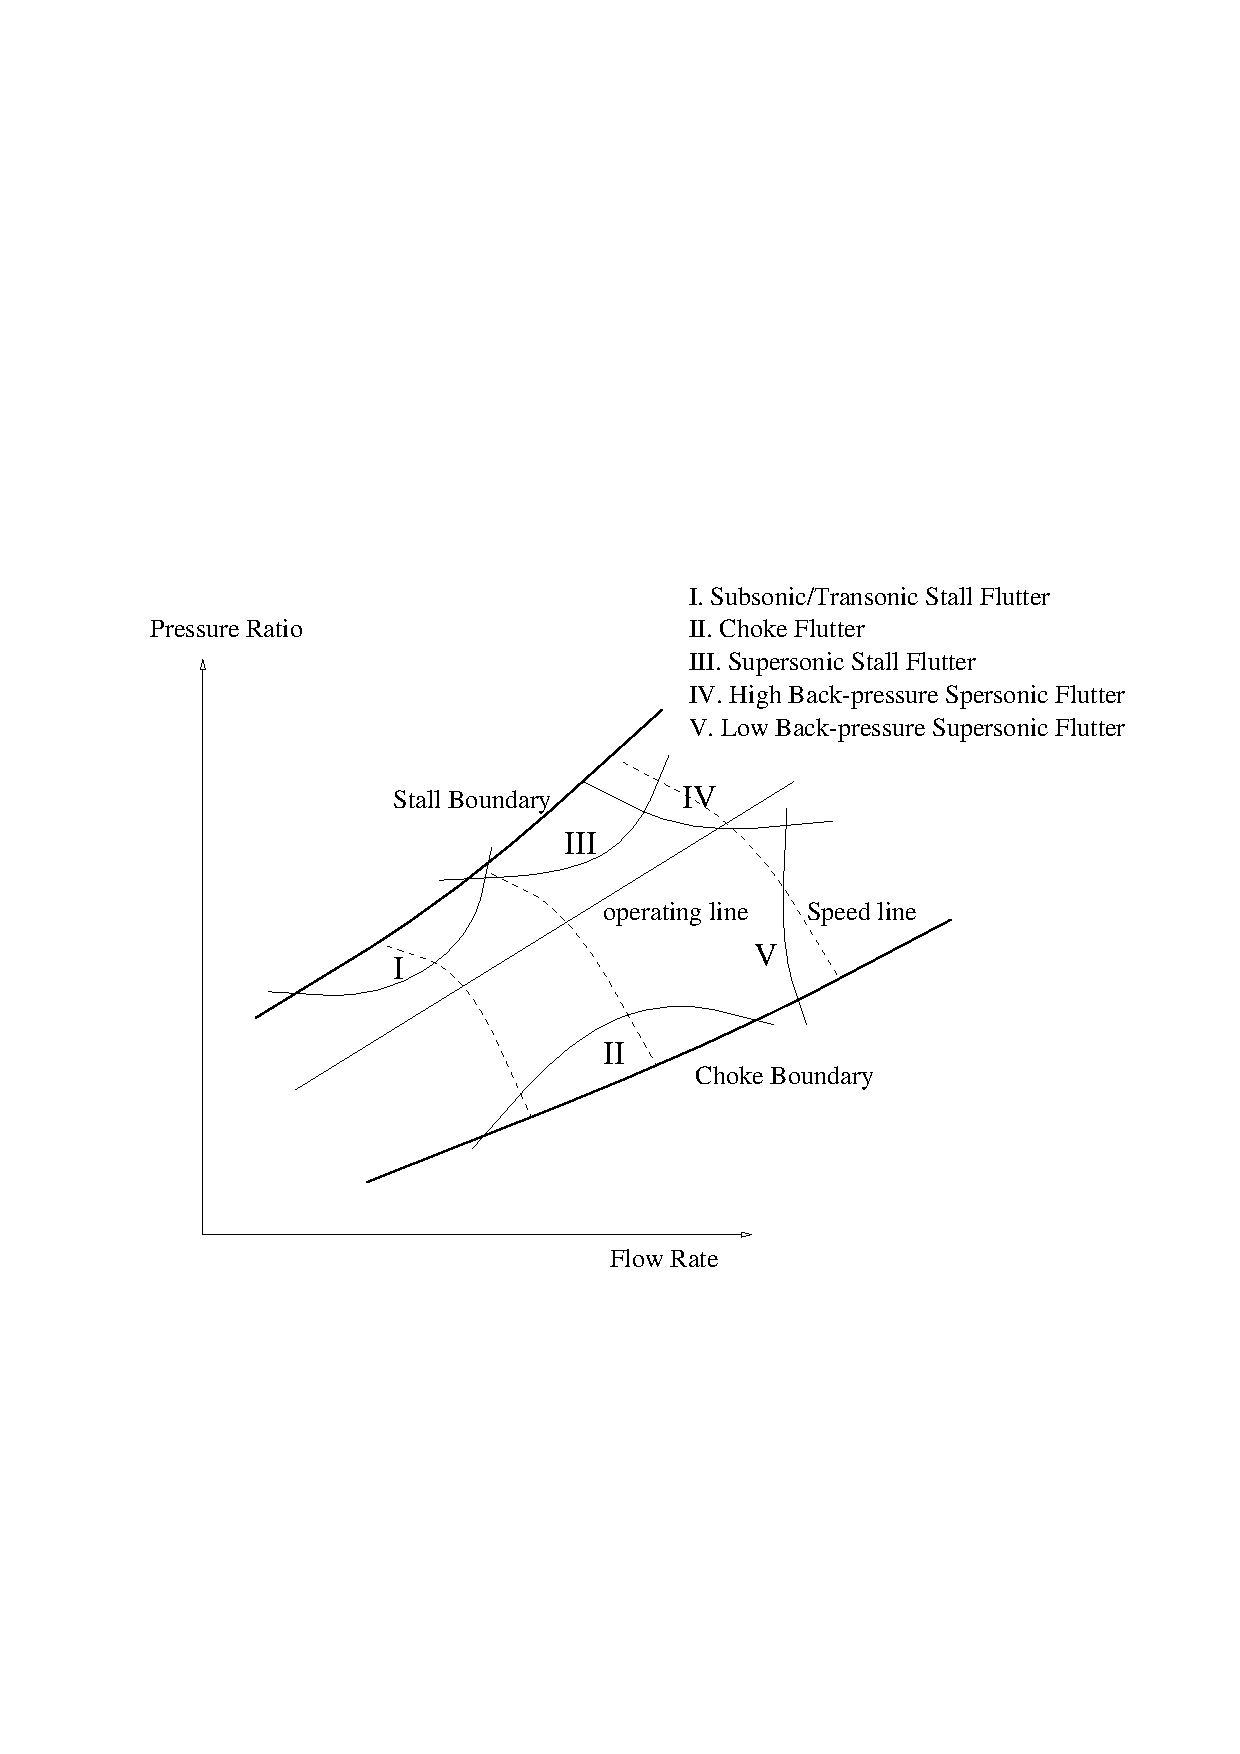
\includegraphics[width=130mm, clip=t]{CHAP_INTRO/FIGURE/fan_map.pdf}}
  \caption{Blade flutter boundaries on compressor map (from Sisto 1987)}
  \label{fan_map.fig}
\end{figure}
%

 A typical compressor map which indicates the different flutter regions
 is shown in Fig. \ref{fan_map.fig}. This map shows the various possible
 flutter regimes: stall flutter, choke flutter and various type of
 supersonic flutter.
 Sisto \citeyear{Sisto:1} gives an overview of the different types of
 flutter in modern compressor and fan. In this review paper
 particular attention as been devoted to the illustration of classical
 and modern prediction models.
%
%
%
\paragraph{Stall flutter.}
%
 As shown in Fig. \ref{fan_map.fig}, the aerodynamic conditions,
 at which stall flutter tends to occur, are at part-speed with high
 back pressure.
 In such conditions, the incidence onto the blades is high and the
 blade boundary layer becomes thicker. At transonic
 flow conditions, which are typical of front stage fans,
 a shock wave stands outside the blade passage, i.e. misses the
 leading-edge of the next blade.
 This leads to strong shock/boundary-layer interaction, which may be an
 important part of the stall flutter mechanism.
 Stall flutter differs considerably from classical flutter,
 i.e. with attached flow (Sisto \citeyearNP{Sisto:2}).
 The mechanism for net energy transfer from the airstream to an oscillating
 blade need not to rely on elastic or aerodynamic coupling between two modes,
 nor upon a phase lag between a displacement and its aerodynamic reaction.
 The essential feature of stall flutter is the non-linear aerodynamic
 reaction to the motion of the blades.
 Dowel et al. \citeyear{Sisto:3} describe a models for bending and torsional
 stall flutter including the basic instability mechanism and its principal
 features.
 Adamczyk et al. \citeyear{Adamczyk:1} present an analysis of supersonic stall
 flutter of modern fan assemblies.
%
%
%
\paragraph{Choke flutter.}
%
 Compared to stall flutter, choke flutter usually occurs at the opposite
 end of the compressor map. Here the incidence onto the blades decreases
 and becomes negative.
 At subsonic flow conditions, this may lead to the separation of the
 boundary layer from the pressure surface, and the flutter mechanism
 is similar to that of stall flutter. At transonic conditions, choke
 will normally occur before stall and large unsteady pressures
 from oscillatory shocks may cause flutter.
 Choke flutter is described qualitatively by Dowel et al. \citeyear{Sisto:3}.

~\newline
 Although low-pressure turbine stages are also known to be prone to flutter
 (Sayma et al. \citeyearNP{Mehdi:5}), fan flutter
 stability is usually considered to be more critical as this component can be
 exposed to effects such as inlet distortion due to gusts, cross-winds and
 foreign object damage. Therefore, a higher flutter margin needs to be
 incorporated into its design.
%
%
%
%
\subsection{Inherent unsteadiness}
%
 Several unsteady phenomena may result from aerodynamic instabilities
 of the fluid. Such instabilities are primarily due to the viscosity
 of the fluid and apply to both turbine and compressor blades.
 Two main aerodynamic instabilities are of concern
 in turbomachinery flows: vortex shedding and rotating stall.
%
\paragraph{Vortex Shedding.}
%
 Trailing edge vortex shedding is a major source of unsteadiness in turbomachinery
 when viscous flow exits via a blunt blade trailing-edge. This unsteadiness
 is particularly pronounced in turbines where very thick trailing-edges are
 needed to accommodate blade cooling passages.
 Some experimental works suggested that the wake loss in a turbine is
 largely due to the formation of a vortex shed.
 Unfortunately, the detailed mechanism of vortex shedding loss production
 is still not quite clear.
 One observation is that, when vortex shedding occurs,
 the total pressure just downstream of the trailing
 edge (base region) is significantly lower than that of the free-stream,
 producing a base pressure loss (Wilson \citeyearNP{Wilson:1}).
 Predicting the base pressure is an important part of predicting the loss
 produced by the vortex shedding. Because vortex shedding in turbomachines
 has a small length scale and high frequency, the experimental and numerical
 investigations are difficult and expensive. However, understanding
 and predicting trailing-edge vortex shedding
 is important to reduce the total losses further in turbine designs
 and is receiving more and more attention.
 Cicarelli \& Sieverding \citeyear{Sieverding:2} present a numerical simulation
 in order to assess the effects of vortex shedding on the unsteady pressure
 distrubution around the trailing-edge of a turbine cascade.
 Magagnato \citeyear{Magagnato:1} uses different forms of two equation
 turbulence models in order to predict the experimentallly observed vortex
 shedding from a turbine trailing edge. The results indicates a strong
 dependency on the particular turbulence model used.
 Denton \citeyear{Denton:2} discusses turbine vortex shedding in term
 of losses due to entropy generation.
%
\paragraph{Rotating stall.}
%
 Stall may occur when a compressor blade runs off design, and the incidence
 on the blade increases (above the working line in Fig. \ref{fan_map.fig}).
 As a consequence, at least three different instabilities may occur:
 the first is stall flutter, described above;
 the second is {\em surge}, where the higher pressure downstream of the stalling
 stage causes the whole flow to reverse. This
 serious system instability can cause structural damage very suddenly.
 The third instability, rotating stall, occurs when, due to differences
 in the flow around the annulus (inlet distortion or upstream obstruction)
 only some of the blades stall.
 The stalled cell then causes a higher incidence onto the blades nearest in the
 opposite direction to the rotation (causing those to stall),
 and a lower incidence onto the blades nearest in the rotating direction
 (causing those to recover).
 Thus the stalled cell rotates around the annulus in the opposite
 direction to the rotor rotation.
 This phenomenon obviously causes large unsteady forces on the blades, so at least
 some forced vibration would be expected to accompany rotating stall.
 The propagative behaviour of rotating stall was initially described by
 Emmons et al. \citeyear{Emmons:1}.
 Advances in the area of rotating stall has been reported by
 Greitzer \citeyear{Greitzer:1,Greitzer:2}, Cumpsty \citeyear{Cumpsty:1}.
%
%
%
%
\subsection{Further aspects of unsteady flows in turbomachines}
%
 There are two main parameters which are of paramount importance in
 turbomachinery unsteady flows and these are the {\em interblade phase angle}
 and the {\em reduced frequency}.
 The interblade phase angle can be associated with both flutter and forced  response problems (stator/rotor interaction). This quantity, firstly
 introduced by Lane \citeyear{Lane:1} for flutter problems,
 indicate the phase difference between vibrating neighboring blades.
 The possible values of the interblade phase angle in a flutter analysis are
 defined by
%
\beq
  \phi = \frac{2 \pi n}{N\sm{b}}
  \label{ibps_flutter}
\eeq
%
 where $N\sm{b}$ represents the number of blade in the annulus and $n$ represents
 the wave number $\left(n = 0, 1, \dots, N\sm{b}\right)$.

 For stator/rotor interaction an equivalent definition can be formulated.
 This time, the interblade phase angle is decided by the pitch ratio
 of neighboring blade rows.
 For example, for a single turbine stage shown in Fig. \ref{turbine_stage.fig},
 the stator blade row has a blade pitch given $P\sm{s} = \frac{2 \pi}{N\sm{s}}$
 and the rotor blade a pitch given by
 $P\sm{r} = \frac{2 \pi}{N\sm{r}}$, where $N\sm{s}$ and $N\sm{r}$ are
 the blade numbers.
 Assuming $N\sm{s} \leq N\sm{r}$, the interblade phase angle between
 the upper and periodic boundaries is:
%
\beq
  \phi = 2 \pi\left(1 - \frac{N\sm{s}}{{N\sm{r}}}\right)
  \label{ibps_forced}
\eeq
%
\begin{figure}[ht]
  \centerline{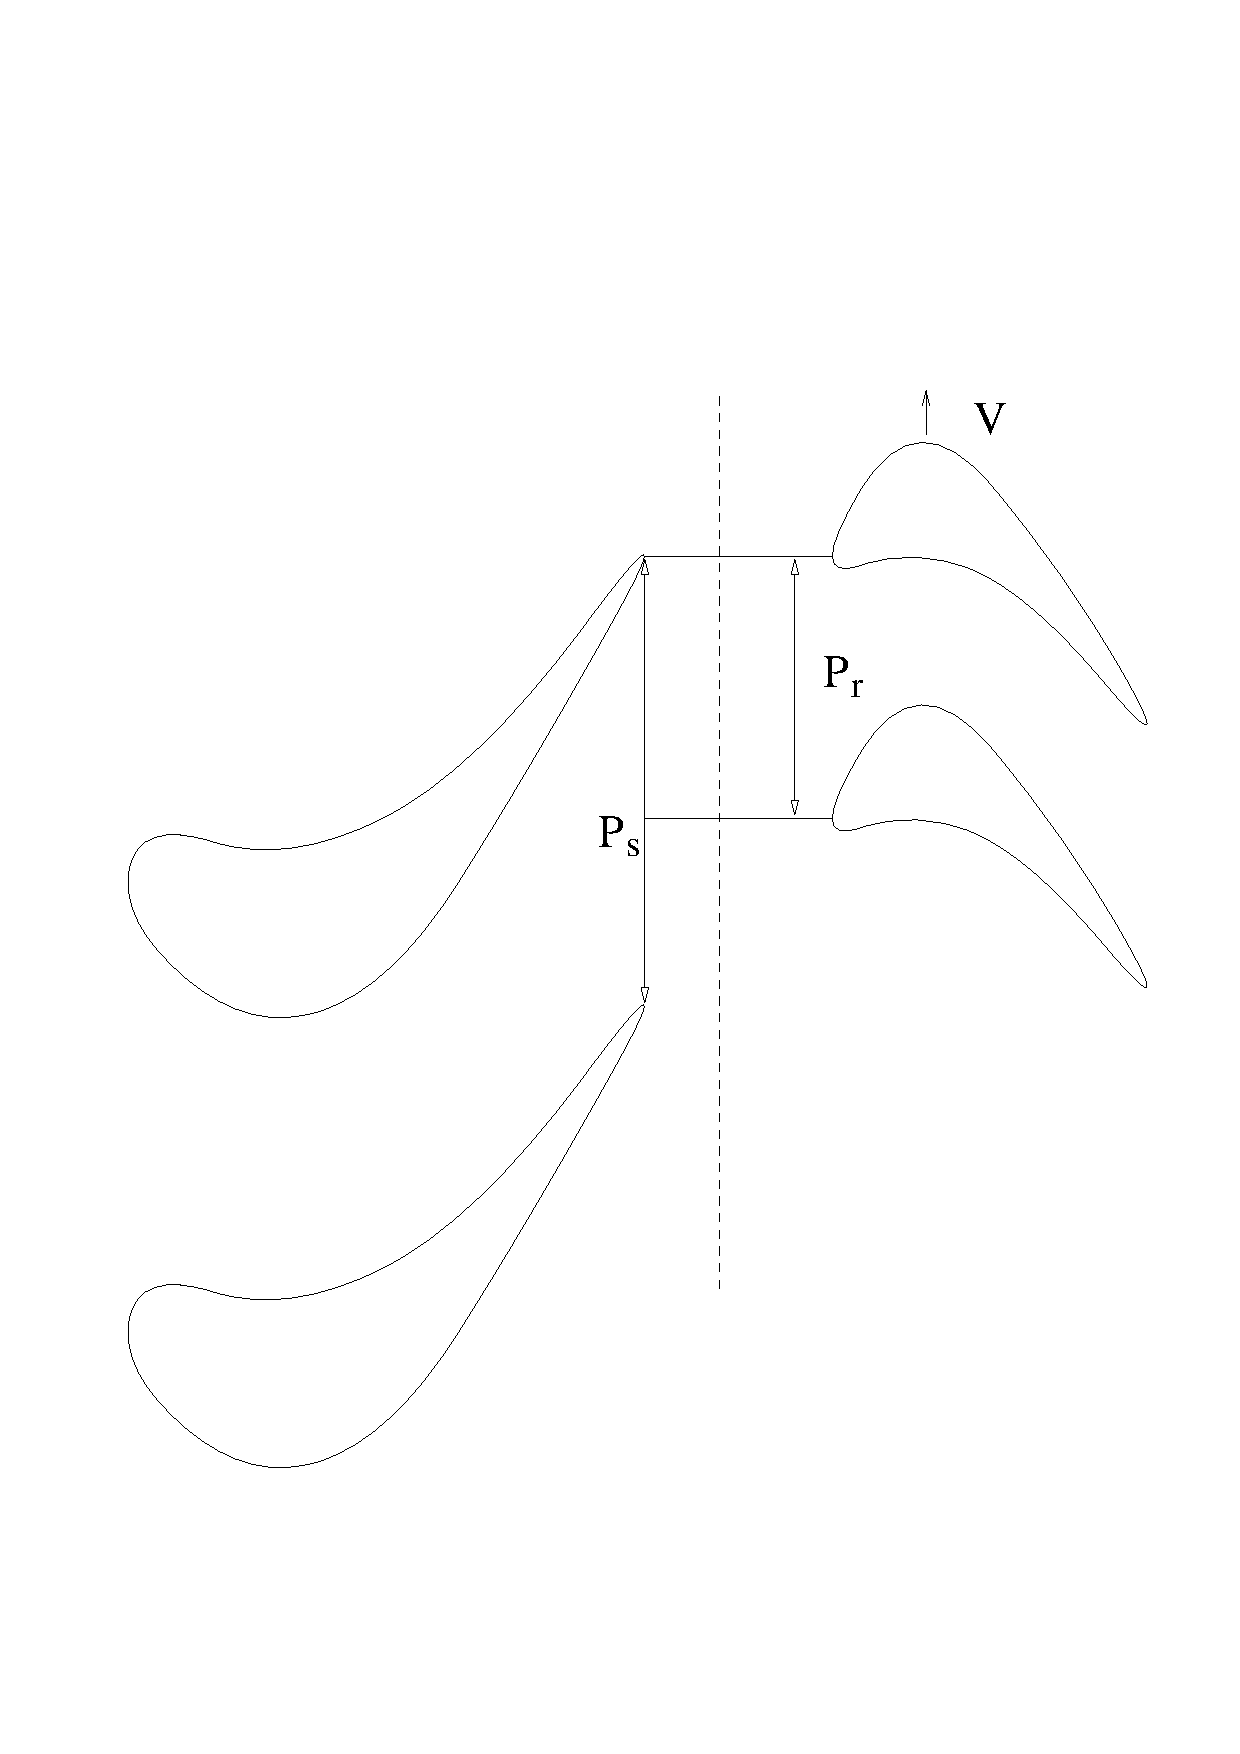
\includegraphics[width=60mm, clip=t]{CHAP_INTRO/FIGURE/turbine_stage.pdf}}
  \caption{Turbine stage with different number of blades in each row}
  \label{turbine_stage.fig}
\end{figure}
%
 The interblade phase angle determinates the number of blade passages that must
 be included in the calculations unless some other assumption
 are introduced to limit the computational domain to a single passage
 (Erdos et al. \citeyearNP{Erdos:1}, Giles \citeyearNP{Giles:2},
  Verdon \citeyearNP{Verdon:2}).

 The reduced frequency is defined in (\ref{reduced_frequency.eq}).
 For stator/rotor interaction the reduced frequency is related to the
 interblade phase angle and the relative rotation speed of the two rows as
 indicated in (\ref{frequency_rotaz.eq}).
 The reduced frequency can be interpreted as the ratio of the time taken
 for a fluid particle to go past the blade chord (or pitch) to the
 period of the flow unsteadiness. For small values
 of the reduced frequency, the flow is quasi-steady, while
 unsteady effects dominate for large values.
%
